\documentclass[aspectratio=169]{beamer}

\usetheme{Boadilla}
\setbeamertemplate{navigation symbols}{}
\setbeamertemplate{footline}[frame number]
\setbeamertemplate{headline}{}
\setbeamercolor{footline}{bg=white,fg=black}
\setbeamercolor{author in head/foot}{bg=white,fg=black}
\setbeamercolor{title in head/foot}{bg=white,fg=black}
\setbeamercolor{date in head/foot}{bg=white,fg=black}

\usepackage{amsmath}
\usepackage{booktabs}
\usepackage{graphicx}
\usepackage{siunitx}
\usepackage{tikz}
\usepackage{pgfplots}
\usepackage{pgfplotstable}
\usetikzlibrary{positioning}
\usepgfplotslibrary{groupplots}

\pgfplotsset{compat=1.18}
\sisetup{
  round-mode=places,
  round-precision=3,
  detect-all
}

\definecolor{coreblue}{HTML}{1F77B4}
\definecolor{socred}{HTML}{D62728}
\definecolor{fpgaorange}{HTML}{FF7F0E}
\definecolor{simgreen}{HTML}{2CA02C}
\definecolor{softgray}{HTML}{666666}

\title{Prometheus SoC}
\subtitle{High-Level Synthesis of a RISC-V Controlled Softmax Accelerator on the PYNQ-Z1}
\author{Jesse Levine}
\institute{Department of Electronics, Carleton University}
\date{\today}

\begin{document}

\begin{frame}
  \titlepage
\end{frame}

\begin{frame}{Motivation}
\begin{itemize}
\item Softmax is small in source code but expensive on a simple integer-oriented processor.
\item The software path must evaluate exponentials, accumulate a global sum, and normalize every output.
\item In fixed-point software, that path is both slow and numerically fragile.
\item The project goal was to replace that bottleneck with dedicated hardware while keeping a small RISC-V core as the system controller.
\end{itemize}
\vspace{2mm}
\textbf{Design question:} is the right endpoint a software-only core, a standalone accelerator, or a tightly integrated SoC?
\end{frame}

\begin{frame}{Project Evolution}
\begin{itemize}
\item Report 1: reproduced the RV32I HLS baseline and the memory-image workflow.
\item Report 2: added the multiplication support needed for practical fixed-point kernels.
\item Report 3: defined the Softmax specialization strategy: shared memory, MMIO control, and approximation-based arithmetic.
\item Report 5: produced the pipelined software baseline and a standalone accelerator.
\item Report 6: integrated both into the final Prometheus SoC.
\end{itemize}
\vspace{2mm}
\textbf{Outcome:} the final result is a system-level architecture choice, not a kernel-only speedup.
\end{frame}

\begin{frame}{System Architecture}
\begin{columns}[T,totalwidth=\textwidth]
\begin{column}{0.58\textwidth}
\centering
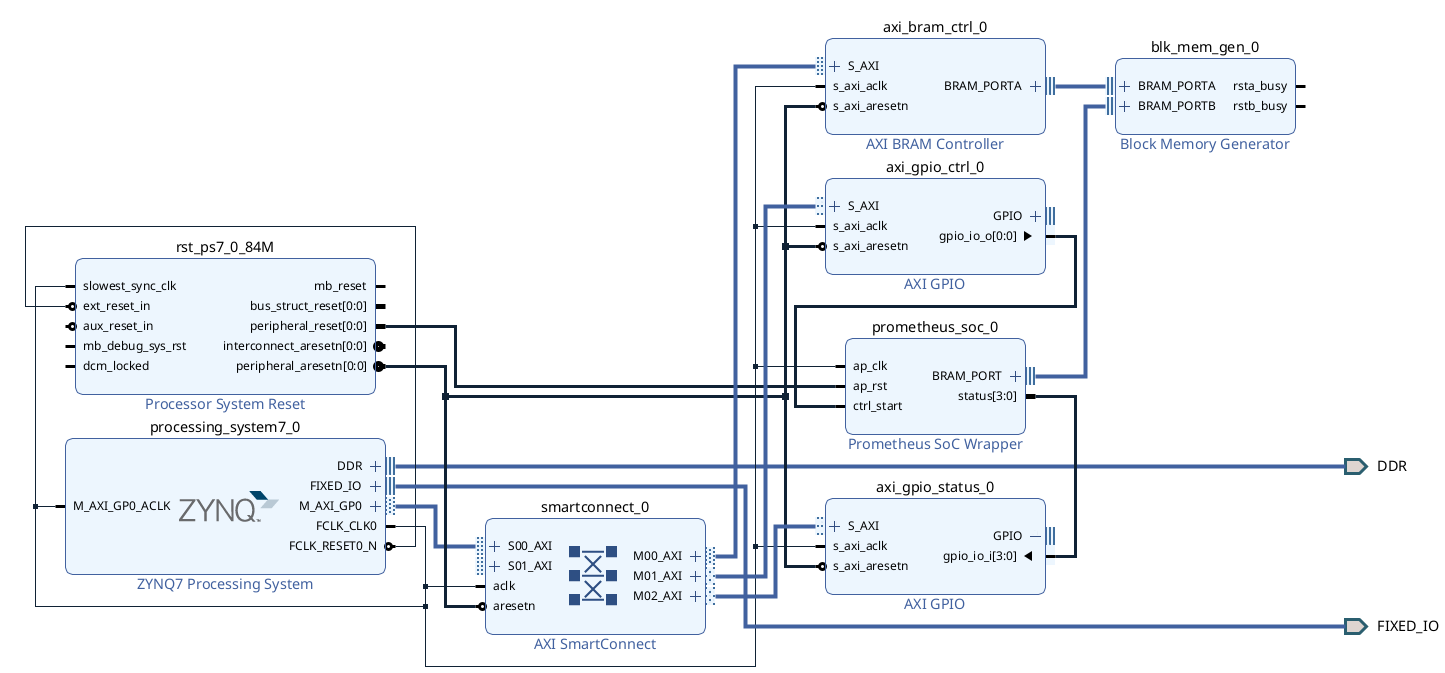
\includegraphics[width=\linewidth]{figures/report6-000.png}
\end{column}
\begin{column}{0.40\textwidth}
\small
\begin{itemize}
\item Zynq PS7 hosts the system and reaches PL through \texttt{M\_AXI\_GP0}.
\item AXI SmartConnect fans out to BRAM control, start GPIO, and status GPIO.
\item Shared BRAM is dual-port and visible to both PS and the HLS SoC wrapper.
\item The wrapper edge-detects start, latches done, and measures cycle count.
\end{itemize}
\end{column}
\end{columns}
\end{frame}

\begin{frame}{Implemented Architecture Summary}
\scriptsize
\begin{tabular}{@{}p{0.27\textwidth}p{0.67\textwidth}@{}}
\toprule
Item & Implemented detail \\
\midrule
Top-level HLS block & One HLS SoC containing a 32-bit RISC-V controller core, a four-lane Softmax accelerator, and a shared BRAM image. \\
Shared memory & 16384 lines $\times$ 128 bits = 256~KiB true dual-port BRAM; each line holds four 32-bit words. \\
Board mapping & PS7 accesses BRAM through AXI at \texttt{0x40000000}; the HLS SoC uses the second BRAM port directly. \\
Local memory map & Program at \texttt{0x0000}; inputs at \texttt{0x4000}; probabilities at \texttt{0x5000}; debug at \texttt{0x6000}; MMIO at \texttt{0x7000}--\texttt{0x7010}. \\
MMIO registers & \texttt{0x7000} AP\_CTRL; \texttt{0x7004} input base; \texttt{0x7008} probability base; \texttt{0x700C} debug base; \texttt{0x7010} vector length $N$. \\
Status word & Bits \texttt{[3:0]} give done, idle, ready, and busy; bits \texttt{[31:4]} hold the latched FPGA cycle count. \\
CPU subset & RV32I integer core plus multiply instructions used by the software path; division and remainder are not implemented. \\
Launch semantics & Writing the MMIO start bit causes the CPU control path to call the accelerator directly and block until completion. \\
\bottomrule
\end{tabular}
\end{frame}

\begin{frame}{Runtime Control Flow}
\centering
\resizebox{0.78\textwidth}{!}{%
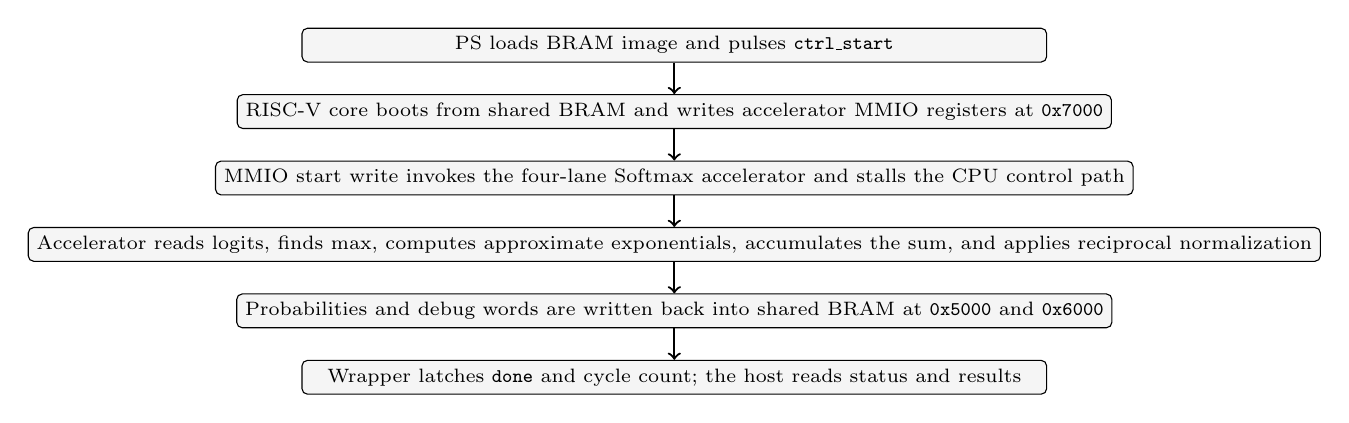
\begin{tikzpicture}[
    node distance=0.40cm,
    flowbox/.style={
        draw,
        rounded corners=2pt,
        align=center,
        font=\scriptsize,
        minimum width=0.78\textwidth,
        inner sep=3pt
    },
    flowarrow/.style={->, thick}
]
\node[flowbox, fill=gray!8] (boot) {PS loads BRAM image and pulses \texttt{ctrl\_start}};
\node[flowbox, fill=gray!8, below=of boot] (cpu) {RISC-V core boots from shared BRAM and writes accelerator MMIO registers at \texttt{0x7000}};
\node[flowbox, fill=gray!8, below=of cpu] (launch) {MMIO start write invokes the four-lane Softmax accelerator and stalls the CPU control path};
\node[flowbox, fill=gray!8, below=of launch] (accel) {Accelerator reads logits, finds max, computes approximate exponentials, accumulates the sum, and applies reciprocal normalization};
\node[flowbox, fill=gray!8, below=of accel] (writeback) {Probabilities and debug words are written back into shared BRAM at \texttt{0x5000} and \texttt{0x6000}};
\node[flowbox, fill=gray!8, below=of writeback] (done) {Wrapper latches \texttt{done} and cycle count; the host reads status and results};

\draw[flowarrow] (boot) -- (cpu);
\draw[flowarrow] (cpu) -- (launch);
\draw[flowarrow] (launch) -- (accel);
\draw[flowarrow] (accel) -- (writeback);
\draw[flowarrow] (writeback) -- (done);
\end{tikzpicture}
}
\end{frame}

\begin{frame}{Accelerator Datapath}
\begin{columns}[T,totalwidth=\textwidth]
\begin{column}{0.54\textwidth}
\small
\begin{itemize}
\item Signed Q16.16 fixed-point datapath
\item Four-lane vector width
\item Maximum supported vector length: 256
\item Stage 1: stream logits and reduce max
\item Stage 2: compute approximate exponentials after max subtraction
\item Stage 3: cache exponentials and accumulate a 64-bit sum
\item Stage 4: apply a 16-segment reciprocal approximation in Q2.30
\item Stage 5: normalize and write probabilities back to BRAM
\end{itemize}
\end{column}
\begin{column}{0.44\textwidth}
\small
\textbf{Approximation strategy}
\begin{equation*}
e^x = 2^{x/\ln 2}
\end{equation*}
\begin{itemize}
\item 17-point piecewise-linear lookup for the fractional exponential term
\item Power-of-two shift for the integer term
\item HLS \texttt{DATAFLOW} to overlap exponentiation, buffering, normalization, and writeback
\end{itemize}
\end{column}
\end{columns}
\end{frame}

\begin{frame}{Implementation-Level Resource Tradeoff}
\begin{columns}[T,totalwidth=\textwidth]
\begin{column}{0.52\textwidth}
\centering
\small
\begin{tabular}{lcc}
\toprule
Resource / Metric & Core Only & SoC \\
\midrule
LUT & 2169 & 26090 \\
FF & 1465 & 52339 \\
DSP & 12 & 32 \\
BRAM & 0 & 9 \\
Post-route period (ns) & 11.345 & 11.514 \\
\bottomrule
\end{tabular}
\end{column}
\begin{column}{0.45\textwidth}
\small
\begin{itemize}
\item The SoC is much larger because it includes the accelerator datapath, local buffers, and the MMIO integration structure.
\item The architectural question is whether this area cost is justified by throughput and numerical gains.
\item The remainder of the results show that the answer is yes.
\end{itemize}
\end{column}
\end{columns}
\end{frame}

\begin{frame}{Latency Scaling}
\begin{columns}[T,totalwidth=\textwidth]
\begin{column}{0.58\textwidth}
\centering
\begin{tikzpicture}
\begin{groupplot}[
    group style={group size=1 by 2, vertical sep=0.95cm},
    width=0.76\linewidth,
    height=3.05cm,
    grid=both,
    grid style={gray!20},
    tick label style={font=\tiny},
    label style={font=\scriptsize}
]
\nextgroupplot[
    ylabel={Core cycles},
    title={Software-only core},
    title style={font=\scriptsize},
    xticklabels=\empty
]
\addplot+[black, mark=*, thick] table[x=n,y=core_cycles,col sep=comma] {data/core_vs_soc.csv};
\nextgroupplot[
    ylabel={SoC cycles},
    xlabel={Sequence length $N$},
    title={Integrated SoC},
    title style={font=\scriptsize}
]
\addplot+[black, mark=square*, thick] table[x=n,y=soc_cycles_sim,col sep=comma] {data/core_vs_soc.csv};
\end{groupplot}
\end{tikzpicture}
\end{column}
\begin{column}{0.38\textwidth}
\small
\begin{itemize}
\item The software-only baseline scales linearly with a very large slope.
\item The integrated SoC keeps the per-element cost extremely small.
\item Separate axes are necessary because a shared axis hides the SoC behavior.
\item This throughput gap is what motivated the final architecture choice.
\end{itemize}
\end{column}
\end{columns}
\end{frame}

\begin{frame}{Numerical Behavior}
\begin{columns}[T,totalwidth=\textwidth]
\begin{column}{0.56\textwidth}
\centering
\begin{tikzpicture}
\begin{axis}[
    width=\linewidth,
    height=5.4cm,
    xlabel={Sequence length $N$},
    ylabel={Softmax sum},
    ymin=0.64,
    ymax=1.02,
    grid=both,
    grid style={gray!20},
    legend style={at={(0.03,0.97)}, anchor=north west, draw=none, fill=none, font=\tiny},
    tick label style={font=\tiny},
    label style={font=\scriptsize}
]
\addplot+[color=coreblue, only marks, mark=*, mark size=1.4pt] table[x=n,y=core_sum,col sep=comma] {data/core_vs_soc.csv};
\addlegendentry{Core only}
\addplot+[color=socred, only marks, mark=square*, mark size=1.4pt] table[x=n,y=soc_sum_sim,col sep=comma] {data/core_vs_soc.csv};
\addlegendentry{Core + accel}
\addplot[dashed, color=softgray] coordinates {(0,1) (140,1)};
\end{axis}
\end{tikzpicture}
\end{column}
\begin{column}{0.40\textwidth}
\small
\begin{itemize}
\item The software-only path loses probability mass as $N$ grows.
\item Its Softmax sum collapses toward roughly $0.675$ for longer vectors.
\item The accelerator-based SoC keeps the sum close to $1.0$.
\item The SoC is therefore not only faster, but also materially better behaved numerically.
\end{itemize}
\end{column}
\end{columns}
\end{frame}

\begin{frame}{Speedup Result}
\begin{columns}[T,totalwidth=\textwidth]
\begin{column}{0.54\textwidth}
\centering
\begin{tikzpicture}
\begin{axis}[
    width=\linewidth,
    height=5.2cm,
    xlabel={Sequence length $N$},
    ylabel={Speedup ratio},
    ymin=0,
    ymax=125,
    grid=both,
    grid style={gray!20},
    tick label style={font=\tiny},
    label style={font=\scriptsize}
]
\addplot+[black, mark=triangle*, thick] table[x=n,y=speedup,col sep=comma] {data/core_vs_soc.csv};
\end{axis}
\end{tikzpicture}
\end{column}
\begin{column}{0.43\textwidth}
\small
\begin{itemize}
\item Measured speedup at $N=128$: \textbf{$114.7\times$}
\item Large-$N$ slope-based limit: \textbf{about $389\times$}
\item The SoC has a larger fixed setup cost.
\item But its marginal cost per additional element is dramatically lower than the software baseline.
\end{itemize}
\end{column}
\end{columns}
\end{frame}

\begin{frame}{FPGA Implementation}
\begin{columns}[T,totalwidth=\textwidth]
\begin{column}{0.50\textwidth}
\centering
\scriptsize
\begin{tabular}{lc}
\toprule
Metric & Implemented SoC \\
\midrule
Board & Digilent PYNQ-Z1 \\
FPGA & \texttt{xc7z020clg400-1} \\
Clock period (ns) & 11.875 \\
Clock frequency (MHz) & 84.211 \\
WNS (ns) & 0.332 \\
WHS (ns) & 0.010 \\
Slice LUTs & 32717 \\
Slice Registers & 60358 \\
Block RAM Tiles & 68.5 \\
DSPs & 32 \\
Timing status & Met \\
\bottomrule
\end{tabular}
\end{column}
\begin{column}{0.46\textwidth}
\small
\begin{itemize}
\item The complete board-integrated design closed timing on the target FPGA.
\item This is not a simulation-only argument: the processor, BRAM, AXI glue, GPIO path, and accelerator were implemented and exercised together.
\item Reported timing values come from the wrapper-level status-word measurement path.
\end{itemize}
\end{column}
\end{columns}
\end{frame}

\begin{frame}{FPGA Validation}
\begin{columns}[T,totalwidth=\textwidth]
\begin{column}{0.49\textwidth}
\centering
\begin{tikzpicture}
\begin{axis}[
    width=\linewidth,
    height=4.1cm,
    xlabel={Sequence length $N$},
    ylabel={Clock cycles},
    grid=both,
    grid style={gray!20},
    tick label style={font=\tiny},
    label style={font=\scriptsize}
]
\addplot+[black, mark=*, thick] table[x=n,y=cycles,col sep=comma] {data/prometheus_soc_n_sweep.csv};
\end{axis}
\end{tikzpicture}
\end{column}
\begin{column}{0.49\textwidth}
\centering
\begin{tikzpicture}
\begin{axis}[
    width=\linewidth,
    height=4.1cm,
    xlabel={Sequence length $N$},
    ylabel={Softmax sum},
    ymin=0.9975,
    ymax=1.001,
    ytick={0.998,0.999,1.000,1.001},
    yticklabel style={/pgf/number format/fixed,/pgf/number format/precision=4},
    grid=both,
    grid style={gray!20},
    tick label style={font=\tiny},
    label style={font=\scriptsize}
]
\addplot+[black, only marks, mark=*, mark size=1.4pt] table[x=n,y=sum,col sep=comma] {data/prometheus_soc_n_sweep.csv};
\addplot[dashed, color=softgray] coordinates {(0,1) (260,1)};
\end{axis}
\end{tikzpicture}
\end{column}
\end{columns}
\vspace{1mm}
\small
FPGA latency remains low across the full sweep, and the Softmax sum stays close to one. At representative points, FPGA cycle counts match simulation exactly.
\end{frame}

\begin{frame}{Takeaways}
\begin{itemize}
\item Prometheus SoC is a tightly integrated RISC-V plus accelerator architecture built with HLS and validated on the PYNQ-Z1.
\item The design uses a shared 128-bit BRAM image, MMIO-controlled launch semantics, and a wrapper that cleanly exposes done and cycle count to the host.
\item The four-lane fixed-point accelerator removes the Softmax bottleneck while also improving numerical behavior relative to the software-only baseline.
\item The final contribution is a complete, measured hardware-software co-design result rather than a standalone accelerator block.
\end{itemize}
\end{frame}

\begin{frame}{References}
\footnotesize
\begin{thebibliography}{9}
\bibitem{toker}
O. Toker, ``A high-level synthesis approach for a RISC-V RV32I-based system on chip and its FPGA implementation,'' \emph{Engineering Proceedings}, 2023.

\bibitem{kim}
R. Kim, D. Lee, J. Kim, J. Park, and S. E. Lee, ``Hardware accelerator for approximation-based softmax and layer normalization in transformers,'' \emph{Electronics}, 2025.

\bibitem{vaswani}
A. Vaswani et al., ``Attention is all you need,'' \emph{NeurIPS}, 2017.
\end{thebibliography}
\end{frame}

\end{document}
